\documentclass[UTF8]{ctexart}
\usepackage{amsmath}
\usepackage{amssymb}
\usepackage{booktabs}
\usepackage{background}
\usepackage{caption, subcaption}
\usepackage{enumitem}
\usepackage{float}
\usepackage{fontspec}
\usepackage{geometry}
\usepackage{mathptmx} %mathptmx和times结合使得公式使用times new roman字体
\usepackage{tikz}
\usepackage{times}
\usepackage{ulem}
\usepackage{xcolor}
\usetikzlibrary{positioning, arrows.meta, shapes.misc}

\geometry{a5paper, top=0.1cm, left=1cm, right=1cm, bottom=1.1cm}
\setCJKmainfont[BoldFont={汉仪文黑-85W},ItalicFont={方正苏新诗柳楷简体}]{汉仪文黑-55W}
\setfontfamily\Issue{Century Schoolbook}
\newCJKfontfamily\TitleFont{思源宋体 CN Heavy}
\newfontfamily\timesnewroman{Times New Roman}
\setmainfont{Times New Roman}
\captionsetup{font=small, labelfont=bf}

\colorlet{darkcyan}{cyan!50!black}
\newcommand\Black[1]{\textcolor[gray]{0.3}{#1}}
\newcommand\Brown[1]{\textcolor[HTML]{998A4E}{#1}}
\newcommand\Emph[1]{\colorbox{cyan!10!}{\textcolor{cyan!50!black}{#1}}}
\newcommand\IssueNumber{13}
\newcommand\Date{2023-12-13}
%\newcommand\Contributer{@金光日}
\newcommand\Subject{离散数学}

\newcommand\A{\text{\slshape\bfseries A}}
\newcommand\B{\text{\slshape\bfseries B}}
\renewcommand\P{\text{\slshape\bfseries P}}

\begin{document}
\backgroundsetup{contents=
\includegraphics{上半示例.png}, center, scale=1, angle=0, opacity=1}
\BgThispage
\begin{center}
{\scriptsize\Issue \textcolor[HTML]{C8BA83}{WEEKLY TIPS}}

{\Huge\bfseries\TitleFont \Black{知\ 识\ 小\ 料}}

\vspace{-0.1cm}
{\footnotesize \Brown{「电计 2203 班」周常规知识整理共享}}
\end{center}

\vspace{-0.5cm}

\begin{figure}[H]
\hspace{1cm}
\begin{minipage}[t]{0.3\textwidth}
\centering
    \Brown{ISSUE.}

    \vspace{-0.6cm}
    \Huge \Issue\slshape\bfseries\Black{\IssueNumber}
\end{minipage}
\hfill
\begin{minipage}[t]{0.3\textwidth}
\centering
    \Brown{日期:\Date} \\
%\vspace{-0.1cm}
%    \Brown{贡献者:\Contributer} \\
\vspace{-0.1cm}
    \Brown{学科:\Subject} \\
\end{minipage}
\hspace{0.8cm}
\end{figure}

\begin{figure}[htb]
\color{cyan!50!black}
\begin{minipage}[c]{0.65\textwidth}
\vspace{0cm}

有向图 $G$ 如右图所示。
\begin{enumerate}[itemsep=0pt, parsep=0pt]
    \item 求 $G$ 的邻接矩阵 $\A$,并求出每一个结点的出度和入度;
    \item 求出 $\A^2$、$\A^3$、$\A^4$,并解释这三个矩阵行、列及对角线各元素的含义,以及给出 $V_2$ 到 $V_1$ 长度小于等于 4 的路径数量;
    \item 求可达矩阵(路径矩阵)$\P$。
\end{enumerate}
\end{minipage}
\begin{minipage}[c]{0.34\textwidth}
\centering

\vspace{0cm}
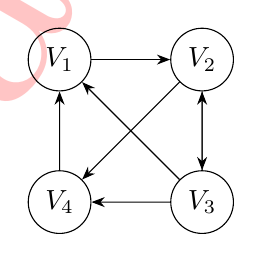
\begin{tikzpicture}[>=Stealth,scale=0.8,->]
    \node[draw, circle] (V1) {$V_1$};
    \node[draw, circle] (V2) [right=of V1] {$V_2$};
    \node[draw, circle] (V3) [below=of V2] {$V_3$};
    \node[draw, circle] (V4) [left= of V3] {$V_4$};
    \draw (V1)--(V2); 
    \draw (V2) -- (V3); 
    \draw (V3)--(V4);
    \draw (V4)--(V1);
    \draw (V2)--(V4);
    \draw (V3)--(V1);
    \draw (V3) --(V2);
\end{tikzpicture}
\end{minipage}
\end{figure}

【第 1 题】邻接矩阵的规则是:两个结点 $V_i,V_j$ 有连边则记 $a_{ij}=1$,否则记为 0。那么,题图的邻接矩阵就不难得到:
\begin{equation}
    \A = \begin{bmatrix} 0&1&0&0 \\ 0&0&1&1 \\ 1&1&0&1 \\ 1&0&0&0  \end{bmatrix}
\end{equation}

通过邻接矩阵来数出度 $d^+$、入度 $d^-$:对第 $i$ 个结点,出度 $d^+(V_i)$ 就是第 $i$ \textbf{行}的 1 的个数,入度 $d^-(V_i)$ 就是第 $i$ \textbf{列}的 1 的个数。或者也可以在图中数出与各个结点相连的边数。得到的结果如下表:
\begin{table}[htb]
  \centering
  \begin{tabular}{ccccc}
  \toprule
    结点 & $V_1$ & $V_2$ & $V_3$ & $V_4$ \\
  \midrule
    出度$d^+$ & 1 & 2 & 3 & 1\\
    入度$d^-$ & 2 & 2 & 1 & 2\\
  \bottomrule
  \end{tabular}
\end{table}
    
【第 2 题】 $\A^2$、$\A^3$、$\A^4$ 使用矩阵乘法的知识即可求出。\textcolor{cyan}{(但也是最容易出错的环节!需要认真+仔细+谨慎)}

\newpage
\backgroundsetup{contents=
\includegraphics{下半示例.png}, center, scale=1, angle=0, opacity=1}
\BgThispage
\begin{equation}
    \A^2 = \begin{bmatrix} 0&0&1&1 \\ 2&1&0&1 \\ 1&1&1&1 \\ 0&1&0&0 \end{bmatrix},\quad
    \A^3 = \begin{bmatrix} 2&1&0&1 \\ 1&2&1&1 \\ 2&2&1&2 \\ 0&0&1&1 \end{bmatrix},\quad
    \A^4 = \begin{bmatrix} 1&2&1&1 \\ 2&2&2&3 \\ 3&3&2&3 \\ 2&1&0&1 \end{bmatrix}
\end{equation}

含义解释:矩阵 $\A^m$ 的第 $i$ 行第 $j$ 列的元素 $a_{ij}^{(m)}$,表示从 $V_i$ 到 $V_j$ 的长度为 $m$ 的不同路径的数目。矩阵 $\A^m$ 的主对角线上元素 $a_{ii}^{(m)}$ 的值,表示结点 $V_i$ 上长度为 $m$ 的圈(回路)的个数。\textcolor{cyan}{(见课本 p334 定理 16.4.1。举个例子,矩阵 $\A^3$ 的 $a_{31}^{(3)}=2$,表示从 $V_3$ 到 $V_1$ 的长度为 3 的路径有 2 条,分别为 $V_3-V_2-V_3-V_1$ 和 $V_3-V_2-V_4-V_1$。)}

从 $V_2$ 到 $V_1$ 的长度小于等于 4 的路径条数,即为 $a_{21} + a_{21}^{(2)} + a_{21}^{(3)} + a_{21}^{(4)} = 0+2+1+2 = 5$。

【第 3 题】可达矩阵的规则是:两个结点 $V_i$ 到 $V_j$ 可达则记 $p_{ij}=1$,否则记为 0。构造方法是:构造 $\B = \A + \A^2 + \A^3 + \A^4$,并将 $\B$ 的所有非零元素改成 1,零元素仍记 0,就得到可达矩阵 $\P$。

换言之,$\A$ 的各次幂矩阵的第 $i$ 行第 $j$ 列的元素 $a_{ij}$、$a_{ij}^{(2)}$、$a_{ij}^{(3)}$、$a_{ij}^{(4)}$ 只要有至少一个不为 0,就把可达矩阵 $\P$ 的对应位置元素 $p_{ij}$ 记为 1;否则记为 0。\textcolor{cyan}{(很幸运,本题中任意两个结点都是可达的,所以可以全部填 1。)}
\begin{equation}
    \P = \begin{bmatrix} 1&1&1&1 \\ 1&1&1&1 \\ 1&1&1&1 \\ 1&1&1&1 \end{bmatrix}
\end{equation}

\textcolor{cyan!80!black}{【结论】见解析。}

\textcolor{cyan!80!black}{【点评】图的矩阵表示包括邻接矩阵、可达矩阵、关联矩阵、权矩阵等,本题考察了最为常见的邻接矩阵和可达矩阵。同学们须弄懂矩阵中元素的含义,以及邻接矩阵的若干次幂的意义。}

\end{document}